\documentclass[ignorenonframetext,]{beamer}
\setbeamertemplate{caption}[numbered]
\setbeamertemplate{caption label separator}{: }
\setbeamercolor{caption name}{fg=normal text.fg}
\beamertemplatenavigationsymbolsempty
\usepackage{lmodern}
\usepackage{amssymb,amsmath}
\usepackage{ifxetex,ifluatex}
\usepackage{fixltx2e} % provides \textsubscript
\ifnum 0\ifxetex 1\fi\ifluatex 1\fi=0 % if pdftex
  \usepackage[T1]{fontenc}
  \usepackage[utf8]{inputenc}
\else % if luatex or xelatex
  \ifxetex
    \usepackage{mathspec}
  \else
    \usepackage{fontspec}
  \fi
  \defaultfontfeatures{Ligatures=TeX,Scale=MatchLowercase}
\fi
% use upquote if available, for straight quotes in verbatim environments
\IfFileExists{upquote.sty}{\usepackage{upquote}}{}
% use microtype if available
\IfFileExists{microtype.sty}{%
\usepackage{microtype}
\UseMicrotypeSet[protrusion]{basicmath} % disable protrusion for tt fonts
}{}
\newif\ifbibliography
\hypersetup{
            pdfborder={0 0 0},
            breaklinks=true}
\usepackage{longtable,booktabs}
\usepackage{caption}
% These lines are needed to make table captions work with longtable:
\makeatletter
\def\fnum@table{\tablename~\thetable}
\makeatother

% Prevent slide breaks in the middle of a paragraph:
\widowpenalties 1 10000
\raggedbottom

\AtBeginPart{
  \let\insertpartnumber\relax
  \let\partname\relax
  \frame{\partpage}
}
\AtBeginSection{
  \ifbibliography
  \else
    \let\insertsectionnumber\relax
    \let\sectionname\relax
    \frame{\sectionpage}
  \fi
}
\AtBeginSubsection{
  \let\insertsubsectionnumber\relax
  \let\subsectionname\relax
  \frame{\subsectionpage}
}

\setlength{\parindent}{0pt}
\setlength{\parskip}{6pt plus 2pt minus 1pt}
\setlength{\emergencystretch}{3em}  % prevent overfull lines
\providecommand{\tightlist}{%
  \setlength{\itemsep}{0pt}\setlength{\parskip}{0pt}}
\setcounter{secnumdepth}{0}
\usepackage[british]{babel}
\usepackage{graphicx,hyperref,anderson,url,booktabs,dcolumn,ragged2e,fixltx2e}
\usepackage{fontawesome}

\title[Sample size determination / Power calculations]{Sample size determination and power calculations for epidemiological research}
\subtitle{Advanced Epidemiology}
\date{April 11, 2017}

\author[Brooke Anderson]{
  Brooke Anderson \\\medskip
  {\small \faEnvelope: \url{brooke.anderson@colostate.edu}} \\
  {\small \faGithub:  \url{www.github.com/geanders}}}

\institute[Colorado State University]{
  Department of Environmental \& Radiological Health Sciences \\
  Environmental Epidemiology Section \\
  Colorado State University}

\date{}

\begin{document}

\begin{frame}
  \titlepage
\end{frame}

\begin{frame}{Course notes and reading}

\begin{block}{Course notes}
A pdf of these coursenotes can be downloaded at: \\ \medskip
\url{https://github.com/geanders/GuestLectures/blob/master/AdvancedEpi/sample_size.pdf}
\end{block}

\begin{block}{Required reading}
Required reading for this lecture is: \\ \medskip
Woodward. 2014. Sample size determination. Chapter 8 of \textit{``Epidemiology: Study Design and Data Analysis."} Third Edition, Chapman \& Hall, Boca Raton, FL. \\ \medskip
Examples in this lecture come from this reading. 
\end{block}

\end{frame}

\begin{frame}{Example: Smoking prevalence in a country}

\begin{block}{Smoking prevalence in a county}
A country's government is interested in determining if the prevalence of smoking among males in the country is 30\%, or if it is higher. They plan to conduct a survey about smoking status in a simple random sample of 5,000 males in the population. A difference in smoking prevalence of 2 percentage points or more would be considered medically significant significant. The government would like to use a test with 5\% significance. Before running the study, the government would like to determine its anticipated power.
\end{block}

\footnotesize{\textit{Sources: Based on an example in Woodward (2014).}}

\end{frame}

\begin{frame}{Example: Smoking prevalence in a country}

\begin{block}{Smoking prevalence in a county}
A country's government is interested in determining \textbf{if the prevalence of smoking among males in the country is 30\%}, or if it is higher. They plan to conduct a survey about smoking status in a simple random sample of 5,000 males in the population. A difference in smoking prevalence of 2 percentage points or more would be considered medically significant significant. The government would like to use a test with 5\% significance. Before running the study, the government would like to determine its anticipated power.
\end{block}

The null hypothesis for the study is that the prevalence of smoking in
the population (\(\pi\)) is 30\%:

\[
H_0 : \pi = \pi_0 = 0.30
\]

\end{frame}

\begin{frame}{Example: Smoking prevalence in a country}

\begin{block}{Smoking prevalence in a county}
A country's government is interested in determining if the prevalence of smoking among males in the country is 30\%, \textbf{or if it is higher}. They plan to conduct a survey about smoking status in a simple random sample of 5,000 males in the population. A difference in smoking prevalence of 2 percentage points or more would be considered medically significant significant. The government would like to use a test with 5\% significance. Before running the study, the government would like to determine its anticipated power.
\end{block}

The alternative hypothesis is that the prevalence of smoking in the
population (\(\pi\)) is higher than 30\%:

\[
H_1 : \pi > 0.30
\]

\end{frame}

\begin{frame}{Example: Smoking prevalence in a country}

\begin{block}{Smoking prevalence in a county}
A country's government is interested in determining if the prevalence of smoking among males in the country is 30\%, or if it is higher. They plan to conduct a survey about smoking status in \textbf{a simple random sample of 5,000 males} in the population. A difference in smoking prevalence of 2 percentage points or more would be considered medically significant significant. The government would like to use a test with 5\% significance. Before running the study, the government would like to determine its anticipated power.
\end{block}

The sample will be a simple random sample, with a sample size (\(n\)) of
5,000:

\[
n = 5000
\]

\end{frame}

\begin{frame}{Example: Smoking prevalence in a country}

\begin{block}{Smoking prevalence in a county}
A country's government is interested in determining if the prevalence of smoking among males in the country is 30\%, or if it is higher. They plan to conduct a survey about smoking status in a simple random sample of 5,000 males in the population. \textbf{A difference in smoking prevalence of 2 percentage points or more would be considered medically significant significant.} The government would like to use a test with 5\% significance. Before running the study, the government would like to determine its anticipated power.
\end{block}

The size of the effect we'd like to detect (\(d\)) is two percentage
points:

\[
d = 0.02
\]

\end{frame}

\begin{frame}{Example: Smoking prevalence in a country}

\begin{block}{Smoking prevalence in a county}
A country's government is interested in determining if the prevalence of smoking among males in the country is 30\%, or if it is higher. They plan to conduct a survey about smoking status in a simple random sample of 5,000 males in the population. A difference in smoking prevalence of 2 percentage points or more would be considered medically significant significant. \textbf{The government would like to use a test with 5\% significance.} Before running the study, the government would like to determine its anticipated power.
\end{block}

The desired Type I error rate (\(\alpha\)) is 5\%:

\[
\alpha = 0.05
\]

\end{frame}

\begin{frame}{Example: Smoking prevalence in a country}

Next, let's think about the hypothesis test that we plan to conduct on
the data that results from this study.

In this case, an appropriate test of this hypothesis is a one-sided test
of proportion. If we use a normal approximation to the binomial
distribution, we can calculate the test statistic as:

\[
z = \frac{p - \pi_0}{\sqrt{\pi_0(1-\pi_0)/n}} = \frac{p - 0.30}{\sqrt{0.30(0.70)/5000}}
\]

We can then compare this z-score to a critical value of
\(z_{0.05} = 1.6449\) (the critical value based on a desired
significance of 5\% for a one-sided hypothesis test). If
\(z > z_{0.05}\), we will reject \(H_0\).

\footnotesize{\textit{If you need a review of this, see Ch. 6.1 of OpenIntro Statistics.}}

\end{frame}

\begin{frame}{Example: Smoking prevalence in a country}

Estimating the power of a study involves some ``what if'' thinking.
Given the parameters of the study design and planned analysis, what
might your data look like and what results might your analysis draw?

The first ``what if'' to lay out are two hypotheses, a \textbf{null
hypothesis} (\(H_0\)), that the true population prevalence is a certain
value (\(\pi_0\)), and a specific \textbf{alternative hypothesis}
(\(H_a\)), that the true population prevalence is a different value
(\(\pi_a\)).

\[ 
H_0 : \pi = \pi_0 = 0.30
\] \[ 
H_a: \pi = \pi_a = \pi_0 + d = 0.32
\]

These hypotheses describe two different scenarios of true smoking
prevalence in the full population. The difference, \(d\), is the size of
the effect we'd like to be able to detect.

\end{frame}

\begin{frame}{Example: Smoking prevalence in a country}

If there were no sampling variation in the prevalence of smoking in a
sample compared to the prevalence in the population, here is how the
survey results of the planned study might look under each of the two
scenarios:

\begin{table}[htbp]
  \centering
  \begin{tabular}{llD{.}{.}{0}D{.}{.}{0}D{.}{.}{0}}
    \toprule && \multicolumn{3}{c}{Smoking status}\\
    \cmidrule{3-3}\cmidrule{4-4}\cmidrule{5-5}Under H\textsubscript{0} && \multicolumn{1}{c}{Yes}&\multicolumn{1}{c}{No}&\multicolumn{1}{c}{Total}\\
    \midrule
    Number &&  1,500 & 3,500 & 5,000 \\
    Proportion && 30\% & 70\% & 100\% \\
    \bottomrule
  \end{tabular}
\end{table}

\begin{table}[htbp]
  \centering
  \begin{tabular}{llD{.}{.}{0}D{.}{.}{0}D{.}{.}{0}}
    \toprule && \multicolumn{3}{c}{Smoking status}\\
    \cmidrule{3-3}\cmidrule{4-4}\cmidrule{5-5}Under H\textsubscript{a} && \multicolumn{1}{c}{Yes}&\multicolumn{1}{c}{No}&\multicolumn{1}{c}{Total}\\
    \midrule
    Number &&  1,600 & 3,400 & 5,000 \\
    Percent && 32\% & 68\% & 100\% \\
    \bottomrule
  \end{tabular}
\end{table}

\end{frame}

\begin{frame}{Example: Smoking prevalence in a country}

However, there \emph{will} be some sampling variation in the measured
prevalence in the surveyed sample of the population compared to the true
prevalence in the whole population.

This sample is large and we can probably assume that sample observations
are independent. We will assume that the sampling distribution of \(p\)
(the prevalence of smoking in the sample) can be approximated by a
normal distribution, centered at the true population prevalence
(\(\pi\)), with standard error of \(\sqrt{\pi(1-\pi)/n}\):

\[
p \sim N\left(\pi, \sqrt{\frac{\pi(1-\pi)}{n}}\right)
\]

\end{frame}

\begin{frame}{Example: Smoking prevalence in a country}

Imagine we conducted 10,000 surveys, each with a random sample of 5,000
men, under the scenarios the prevalence in the true population was
either 0.30 (\(H_0\)) or 0.32 (\(H_a\)). Here are histograms of how the
estimated prevalence in the samples might be distributed:

\begin{center}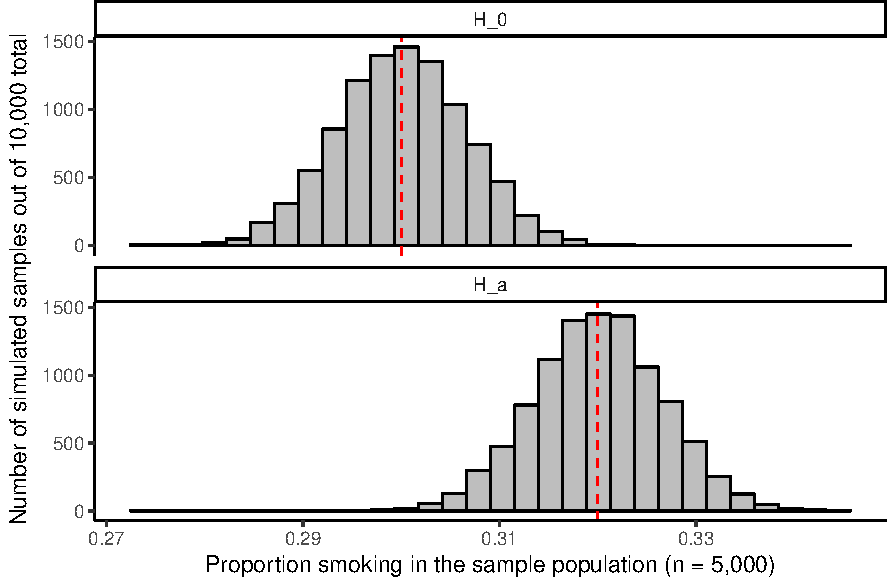
\includegraphics[height=0.6\textheight]{sample_size_files/figure-beamer/unnamed-chunk-1-1} \end{center}

\end{frame}

\begin{frame}{Example: Smoking prevalence in a country}

Because of this sampling variation, under the \(H_0\) scenario our study
data could easily look like this:

\begin{table}[htbp]
  \centering
  \begin{tabular}{llD{.}{.}{0}D{.}{.}{0}D{.}{.}{0}}
    \toprule && \multicolumn{3}{c}{Smoking status}\\
    \cmidrule{3-3}\cmidrule{4-4}\cmidrule{5-5}Under H\textsubscript{0} && \multicolumn{1}{c}{Yes}&\multicolumn{1}{c}{No}&\multicolumn{1}{c}{Total}\\
    \midrule
    Number &&  1,520 & 3,480 & 5,000 \\
    Proportion && 30.4\% & 69.6\% & \\
    \bottomrule
  \end{tabular}
\end{table}

or this:

\begin{table}[htbp]
  \centering
  \begin{tabular}{llD{.}{.}{0}D{.}{.}{0}D{.}{.}{0}}
    \toprule && \multicolumn{3}{c}{Smoking status}\\
    \cmidrule{3-3}\cmidrule{4-4}\cmidrule{5-5}Under H\textsubscript{0} && \multicolumn{1}{c}{Yes}&\multicolumn{1}{c}{No}&\multicolumn{1}{c}{Total}\\
    \midrule
    Number &&  1,470 & 3,530 & 5,000 \\
    Proportion && 29.4\% & 70.6\% & \\
    \bottomrule
  \end{tabular}
\end{table}

\end{frame}

\begin{frame}{Example: Smoking prevalence in a country}

While under the \(H_a\) scenario, our study data could easily look like
this:

\begin{table}[htbp]
  \centering
  \begin{tabular}{llD{.}{.}{0}D{.}{.}{0}D{.}{.}{0}}
    \toprule && \multicolumn{3}{c}{Smoking status}\\
    \cmidrule{3-3}\cmidrule{4-4}\cmidrule{5-5}Under H\textsubscript{a} && \multicolumn{1}{c}{Yes}&\multicolumn{1}{c}{No}&\multicolumn{1}{c}{Total}\\
    \midrule
    Number &&  1,655 & 3,345 & 5,000 \\
    Proportion && 33.1\% & 66.9\% & \\
    \bottomrule
  \end{tabular}
\end{table}

or this:

\begin{table}[htbp]
  \centering
  \begin{tabular}{llD{.}{.}{0}D{.}{.}{0}D{.}{.}{0}}
    \toprule && \multicolumn{3}{c}{Smoking status}\\
    \cmidrule{3-3}\cmidrule{4-4}\cmidrule{5-5}Under H\textsubscript{a} && \multicolumn{1}{c}{Yes}&\multicolumn{1}{c}{No}&\multicolumn{1}{c}{Total}\\
    \midrule
    Number &&  1,560 & 3,440 & 5,000 \\
    Proportion && 31.2\% & 68.8\% & \\
    \bottomrule
  \end{tabular}
\end{table}

\end{frame}

\begin{frame}{Example: Smoking prevalence in a country}

Next, we can apply our planned analysis to the data in each of the
20,000 simulated surveys. For each simulated survey, we can measure
\(p\) (prevalence of smoking in the sample) and then calculate the test
statistic (\(z\)):

\[
z = \frac{p - \pi_0}{\sqrt{\pi_0(1-\pi_0)/n}} = \frac{p - 0.30}{\sqrt{0.30(0.70)/5000}}
\]

We can then compare this z-score to a critical value of
\(z_{0.05} = 1.6449\) (the critical value based on a desired
significance of 5\% for a one-sided hypothesis test). If
\(z > z_{0.05}\), we will reject \(H_0\).

\end{frame}

\begin{frame}{Example: Smoking prevalence in a country}

Here are the simulated samples again, but this time the color shows
which samples result in a rejection of \(H_0\):

\begin{center}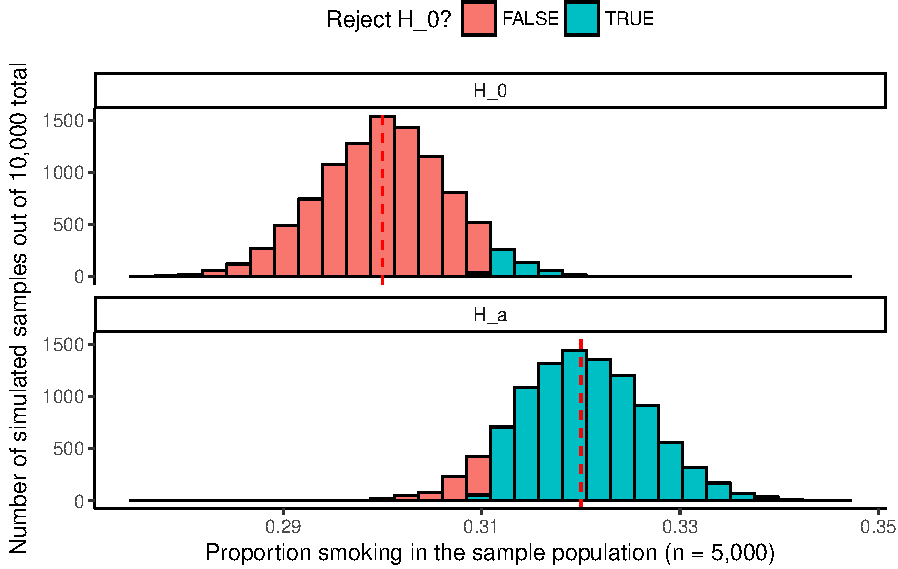
\includegraphics[height=0.7\textheight]{sample_size_files/figure-beamer/unnamed-chunk-2-1} \end{center}

\end{frame}

\begin{frame}{Example: Smoking prevalence in a country}

In these simulated samples, we can measure the percent of samples that
rejected the null under each scenario (\(H_0\) and \(H_a\)):

\begin{longtable}[]{@{}ccc@{}}
\toprule
Scenario & \% failing to reject H\_0 & \% rejecting H\_0\tabularnewline
\midrule
\endhead
H\_0 & 95.4\% & 4.6\%\tabularnewline
H\_a & 7.6\% & 92.4\%\tabularnewline
\bottomrule
\end{longtable}

\begin{itemize}
\tightlist
\item
  The \textbf{Type I error rate} (\(\alpha\)) of our planned study is
  about 5\%
\item
  The \textbf{Type II error rate} (\(\beta\)) of our planned study is
  about 8\%
\item
  The \textbf{power} *(\(1 - \beta\)) of our planned study is about 92\%
\end{itemize}

\end{frame}

\begin{frame}{Example: Smoking prevalence in a country}

We can expand this ``what if'' exercise to see what power we would
expect for different sample sizes. For different sample sizes between
100 and 10,000, we can simulate sample data for many samples from the
population under the \(H_a\) scenario and figure out in what percent of
these samples we would reject \(H_0\).

The result is a \textbf{power curve}:

\begin{center}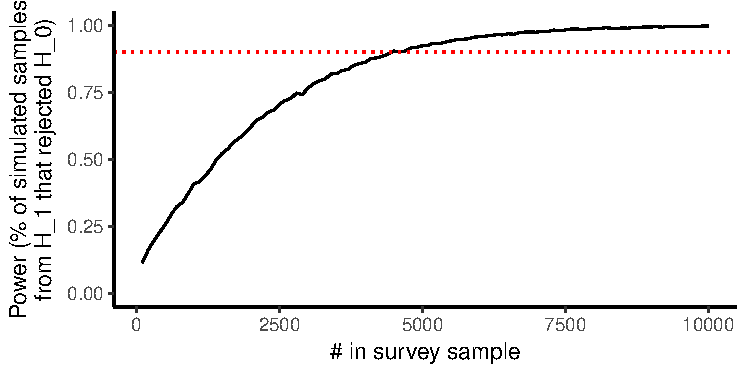
\includegraphics[width=0.8\textwidth]{sample_size_files/figure-beamer/unnamed-chunk-4-1} \end{center}

\end{frame}

\begin{frame}{Hypothesis testing-- A brief review}

\begin{columns}
\begin{column}{0.65\textwidth}
\begin{block}{Hypothesis testing}
\begin{enumerate}
  \item Establish a null hypothesis.
  \item Collect sample data to test that null hypothesis.
  \item Calculate an appopriate \textit{test statistic} given the study design and hypothesis test (e.g., z-score).
  \item Compare the test statistic to to an appropriate \textit{critical value}, based on a predetermined level of significance and using a critical value from the appropriate distribution.
  \item If the test statistic is more extreme than the critical value, reject the null hypothesis.
\end{enumerate}
\end{block}
\end{column}

\begin{column}{0.35\textwidth}

\begin{center}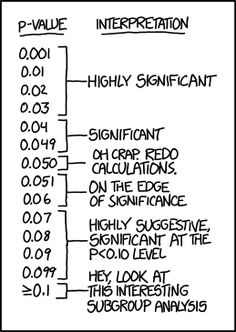
\includegraphics[width=\textwidth]{images/p_values} \end{center}
\footnotesize{Source: \url{http://xkcd.com}}
\end{column}
\end{columns}

\end{frame}

\begin{frame}{Hypothesis testing-- A brief review}

\begin{columns}
\begin{column}{0.5\textwidth}

\begin{center}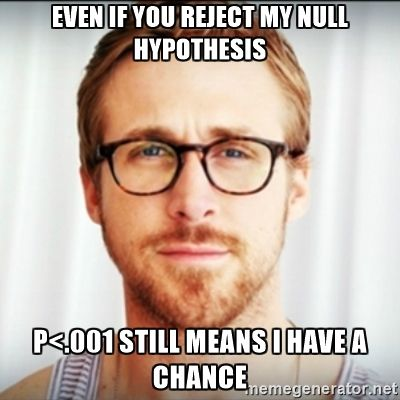
\includegraphics[width=\textwidth]{images/reject_null} \end{center}
\end{column}

\begin{column}{0.5\textwidth}
\begin{block}{Hypothesis tests are not infallible}
\begin{itemize}
  \item Occasionally, a study will reject the null hypothesis when the population value is the null value. 
  \item Occasionally, a study will fail to reject the null hypothesis when the population value has an effect equal or larger than the effect size to be detected. (Bland and Altman: ``Absence of evidence is not evidence of absence.")
\end{itemize}
\end{block}
\end{column}
\end{columns}

\end{frame}

\begin{frame}{Type I and Type II errors}

There are two ways to be wrong in a hypothesis test:

\begin{center}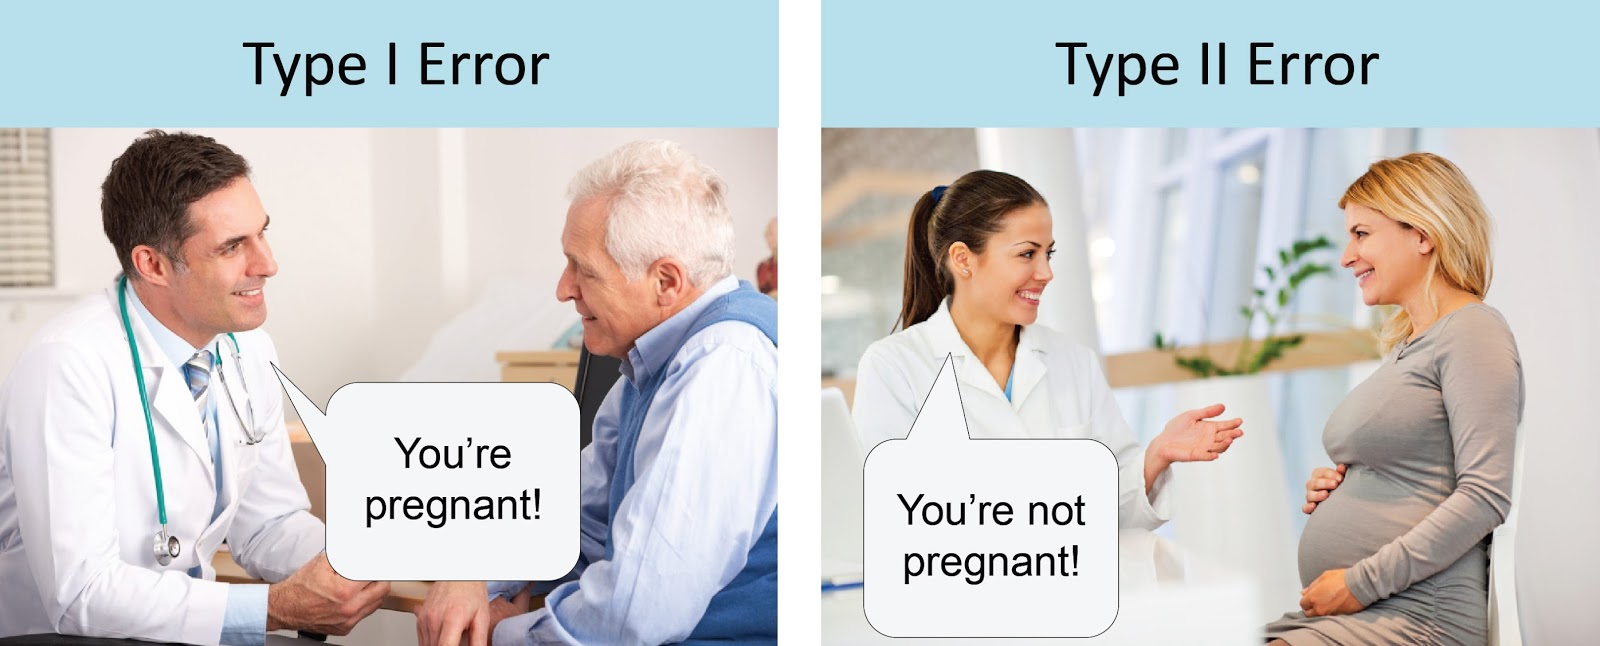
\includegraphics[width=0.8\textwidth]{images/error_types} \end{center}

\begin{itemize}
\tightlist
\item
  Type I error: Reject the null hypothesis when the null hypothesis is
  true
\item
  Type II error: Accepting the null hypothesis when the null hypothesis
  is false
\end{itemize}

\footnotesize{Figure source: \url{http://unbiasedresearch.blogspot.com}}

\end{frame}

\begin{frame}{Type I and Type II errors}

Revisiting our simulated samples for the smoking prevalence example, we
can divide the samples into three groups:

\begin{itemize}
\tightlist
\item
  No error: Red in the samples from the \(H_0\) scenario and blue in the
  samples from the \(H_a\) scenario
\item
  Type I error: Blue in the samples from the \(H_0\) scenario
\item
  Type II error: Red in the samples from the \(H_a\) scenario
\end{itemize}

\begin{center}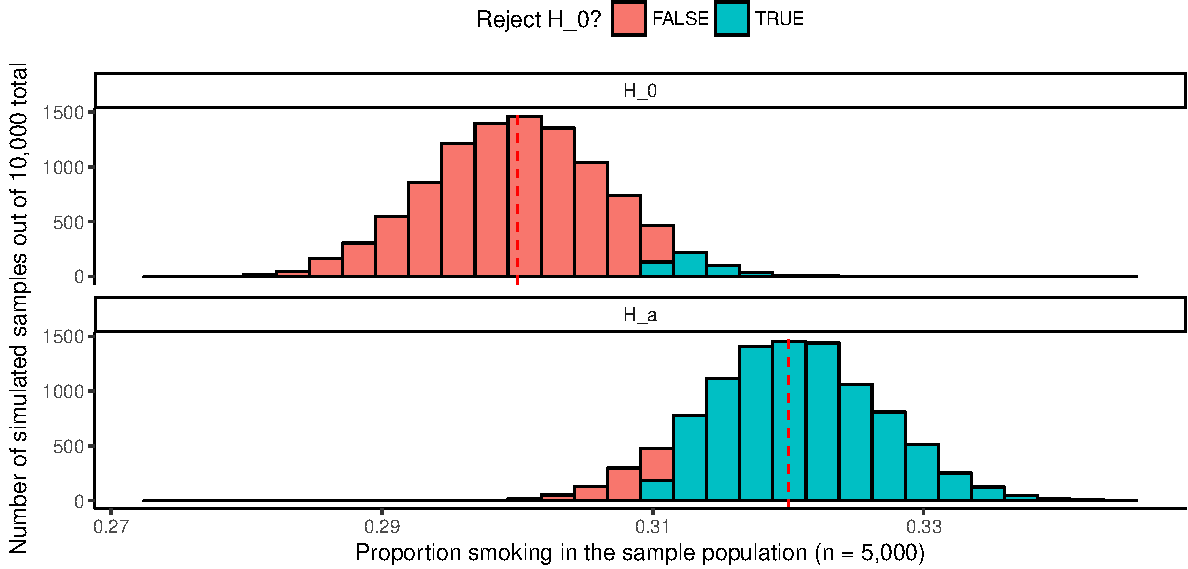
\includegraphics[height=0.5\textheight]{sample_size_files/figure-beamer/unnamed-chunk-8-1} \end{center}

\end{frame}

\begin{frame}{Definition of power}

\begin{block}{Definition of ``power"}
In statistical studies, the \textbf{power} of a hypothesis test is \textbf{the probability of rejecting the null hypothesis when the null hypothesis is false. It is one minus the Type II error rate.} 
\end{block}

A hypothesis test's power typically varies with:

\begin{itemize}
\tightlist
\item
  The design of the study and planned analysis (including if the
  hypothesis test will be one-sided or two-sided)
\item
  The size of the effect being tested
\item
  The desired Type I error rate for the test
\item
  The number of observations
\item
  Variation in observations
\end{itemize}

Depending on the study design and planned analysis, there are also other
factors than can affect power.

\end{frame}

\begin{frame}{Why calculate power?}

If we conduct a study with low power (an \emph{underpowered study}) in
the example study, we would be likely to fail to reject the null
hypothesis even when the true prevalence of smoking in the population is
meaningfully higher than 30\%.

If we conduct a study with extremely high power (an \emph{overpowered
study}) in the example study, we would survey many more people than we
need to and the study would be more expensive than necessary.

\begin{itemize}
\tightlist
\item
  Too few samples is a total waste
\item
  Too many samples is a partial waste
\end{itemize}

\footnotesize{Adapted from Karl Broman, \url{https://www.biostat.wisc.edu/~kbroman/talks/acuc_ho.pdf}}

\end{frame}

\begin{frame}{Why calculate power?}

For the example of estimating smoking prevalence, what would we expect
if we planned to survey 500 people instead of 5,000?

\begin{center}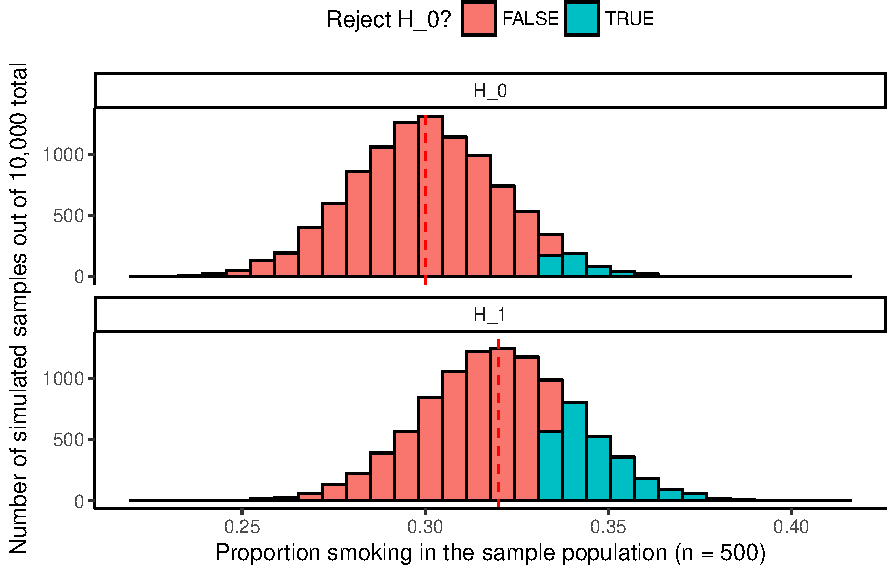
\includegraphics[height=0.7\textheight]{sample_size_files/figure-beamer/unnamed-chunk-9-1} \end{center}

\end{frame}

\begin{frame}{Why calculate power?}

\begin{itemize}
\tightlist
\item
  A study that is underpowered is unlikely to be funded.
\item
  A study that is overpowered may detect results that are statistically
  significant but not medically significant.
\item
  There are ethical reasons to avoid conducting both underpowered and
  overpowered studies.
\item
  Power calculations are often required in grant proposals and for IRB
  approval.
\item
  Including a power calculation in the design phase of an experiment can
  help with optimizing the study design.
\end{itemize}

\end{frame}

\begin{frame}{Why calculate power?}

If a research area is prone to underpowered studies, it can threaten the
reliability of research in that field:

\begin{itemize}
\tightlist
\item
  Publication bias is more likely with underpowered studies
\item
  A study that is underpowered has a lower \emph{positive predictive
  value} (i.e., a reduced probability that the effect is real if the
  null is rejected)
\item
  Effect sizes from underpowered studies that reject the null are likely
  to be inflated (\emph{Winners' curse})
\end{itemize}

\footnotesize{Button et al. (2013) Power failure: why small sample size undermines the reliability of neuroscience. \textit{Nature Reviews} 14:365--376.}

\end{frame}

\begin{frame}{Ways to increase a study's power}

\begin{columns}
\begin{column}{0.6\textwidth}
\begin{block}{Ways to increase a study's power}
\begin{itemize}
  \item Increase number of observations.
  \item Increase the effect size to be detected.
  \item Accept a higher Type I error rate. 
  \item Decrease variance in observations.
\end{itemize}
\end{block}
\end{column}

\begin{column}{0.4\textwidth}

\begin{center}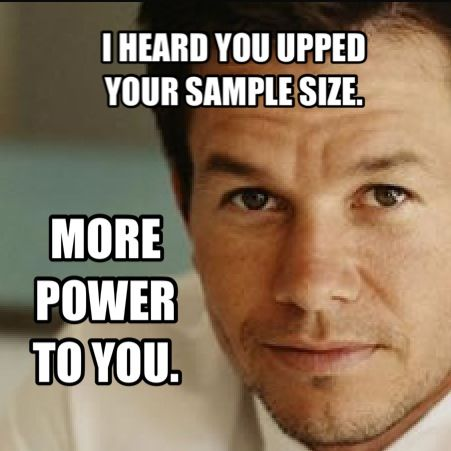
\includegraphics[width=\textwidth]{images/sample_size} \end{center}
\end{column}
\end{columns}

\end{frame}

\begin{frame}{Related calculations}

You can estimate the value of any of these elements while holding the
others constant:

\begin{itemize}
\tightlist
\item
  \textbf{Power}: Given set values for effect size, Type I error rate,
  sample size, and variation in measurements, how likely will the study
  be to reject the null hypothesis when the null hypothesis is false?
\item
  \textbf{Sample size determination}: Given set values for effect size,
  Type I error rate, power, and variation in measurements, how many
  observations (samples) do you need?
\item
  \textbf{Minimum detectable difference}: Given set values for the
  sample size, Type I error rate, power, and variation in measurements,
  what is the smallest effect size you are likely to be able to detect?
\end{itemize}

\end{frame}

\begin{frame}{Tools for calculating power}

There are a number of tools available for calculating power, including:

\begin{itemize}
\tightlist
\item
  Formulae (evaluate ``by hand'')
\item
  Sample size tables
\item
  Software
\item
  Rules of thumb
\item
  Simulations
\end{itemize}

With all these tools, it is critical to remember that you must select a
tool that is appropriate for the study design and the analysis you plan
to conduct. Also keep in mind that, for a very complex analysis, there
may not be an available method for calculating power.

\end{frame}

\begin{frame}{Formulae}

Formulae that can be calculated by hand exist for many simple hypothesis
tests that use a normal distribution or approximation, including:

\begin{itemize}
\tightlist
\item
  Test of a single proportion
\item
  Test of a single mean
\item
  Test of difference between two means in unpaired data
\item
  Test of difference between two means in paired data
\item
  Test of difference in proportions in unmatched data
\item
  Test of difference in proportions in matched data
\end{itemize}

\begin{block}{}
\begin{quotation}"Most hand calculations diabolically strain human limits, even for the easiest formula."\end{quotation}

\footnotesize{Schulz and Grimes. (2005) Sample size calculations in randomised trials: mandatory and mystical. \textit{Lancet} 365:1348--53.}
\end{block}

\end{frame}

\begin{frame}{Formulae-- Test of a single proportion}

For a one-sided hypothesis test of a single proportion, a z-score for
Type II error, \(z_{\beta}\), can be calculated as:

\[
z_{\beta} = \frac{d\sqrt{n}-z_{\alpha}\sqrt{\pi_0(1-\pi_0)}}{\sqrt{\pi_1(1 - \pi_1)}}
\]

where \(\pi_0\) is the population proportion under the null hypothesis,
\(\pi_1\) is the population proportion under the alternative hypothesis,
\(d\) is the difference you wish to detect (\(\pi_1 - \pi_0\)), \(n\) is
the sample size, and \(z_{\alpha}\) is the critical value based on the
desired Type I error rate. You can compare \(z_{\beta}\) to a standard
normal distribution to get \(\beta\) and then calculate \(1 - \beta\) to
determine power.

\end{frame}

\begin{frame}{Example: Smoking prevalence in a country}

For the smoking prevalence example we started the lecture with, this
equation becomes:

\[
z_{\beta} = \frac{d\sqrt{n}-z_{\alpha}\sqrt{\pi_0(1-\pi_0)}}{\sqrt{\pi_1(1 - \pi_1)}}
\]

\[
z_{\beta} = \frac{0.02\sqrt{5000}-1.64\sqrt{0.30(1-0.30)}}{\sqrt{0.32(1 - 0.32)}} = 1.42
\]

This value for \(z_{\beta}\) results in an estimated power of 92.2\% for
the planned study. This calculated power estimate agrees with the value
we estimated from the simulation earlier in the lecture.

\end{frame}

\begin{frame}{Example: Smoking prevalence in a country}

You can use this equation to create a power curve of sample size as a
function of power, holding \(\pi_0\), \(\pi_1\), and \(z_{\alpha}\)
constant:

\begin{center}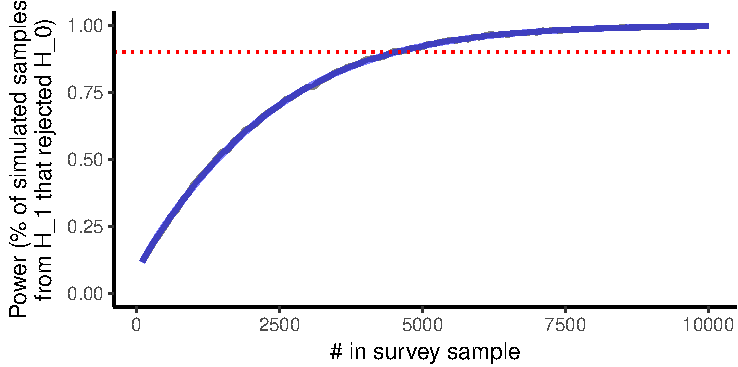
\includegraphics[width=0.8\textwidth]{sample_size_files/figure-beamer/unnamed-chunk-11-1} \end{center}

\end{frame}

\begin{frame}{Formulae-- Test of a single proportion}

If you rearrange this equation, you can also get an equation for
determing the sample size required given a desired power (all constants
are defined as in the previous equation):

\[
n = \frac{1}{d^2}\left(z_{\alpha}\sqrt{\pi_0(1-\pi_0)} + z_{\beta}\sqrt{\pi_1(1-\pi_1)}\right)^2
\]

The reading for today's course includes the formulae for power
calculations, and examples of their use, for a number of other
hypothesis tests.

\end{frame}

\begin{frame}{Software}

There are several software programs that can be used to calculate power
for some types of study designs and planned analysis. These include
functions within more general software (e.g., SAS, Stata, R) and
programs more customized to power calculations. Some options are:

\begin{itemize}
\tightlist
\item
  OpenEpi (\url{http://www.openepi.com/Menu/OE_Menu.htm})
\item
  Epi Info (\url{https://www.cdc.gov/epiinfo/index.html})
\item
  NQuery Advisor (from \url{https://www.statcon.de/})
\item
  PASS (\url{http://www.ncss.com/pass.html})
\end{itemize}

\end{frame}

\begin{frame}{Software}

Advantages of using software include:

\begin{itemize}
\tightlist
\item
  Many of the formulae for power calculations can ``diabolically strain
  human limits'' (Shulz and Grimes)
\item
  Many of the formulae require normal approximations, while software can
  allow exact methods
\end{itemize}

However, it is \textbf{critical} to remember that there are many
different equations for calculating power, and when using software you
\textbf{must} pick the appropriate one for the planned study design and
analysis.

Also, note that statistical power calculations tend to be limited to
simpler study designs and hypothesis tests.

\end{frame}

\begin{frame}{Software}

Using software for a power calculation must be done thoughtfully. When
using software for a power calculation, you should take the following
steps:

\begin{itemize}
\tightlist
\item
  Identify your study design
\item
  Outline the hypothesis test you plan to conduct on the resulting data
\item
  Determine if there is software to conduct a power analysis for that
  type of study design and hypothesis test
\item
  Collect required information to input in software
\item
  Read software documentation closely to determine the assumptions and
  methods used by the software for the power calculation you are
  conducting
\item
  Plug the required inputs into the software to generate an estimate of
  the study's power (or required sample size or minimum detectable
  difference)
\end{itemize}

\end{frame}

\begin{frame}{Required information-- Testing a relative risk in a cohort
study}

The required inputs for a power calculation or sample size determination
for a hypothesis test comparing two proportions (e.g., a test of a
relative risk) for a cohort study, cross-sectional survey, or randomized
clinical trial are (you need all but one):

\begin{itemize}
\tightlist
\item
  Proportion (risk) in unexposed
\item
  Proportion (risk) in exposed \emph{or} risk ratio
\item
  Sample size in unexposed and in exposed \emph{or} ratio of unexposed
  to exposed in the sample
\item
  Desired Type I error rate
\item
  Desired power
\end{itemize}

\end{frame}

\begin{frame}{Software-- Example}

\begin{block}{Cohort study of smoking and heart disease}
A research group is going to conduct a cohort study of smoking and death from coronary heart disease (CHD) in men, selecting a random sample of men from the population of interest. The men will be surveyed about smoking status and then monitored over 5 years for relevant health outcomes. The researchers would like to be 90\% sure of detecting a relative risk for CHD of 1.4 for smokers versus non-smokers, using a two-sided test with 5\% significance. Based on the literature, non-smokers have a average annual CHD death rate of 413 per 100,000. Assuming equal numbers of smokers and non-smokers will be surveyed, what should the total sample size be?
\end{block}

\footnotesize{\textit{Source: Based on an example in Woodward (2014).}}

\end{frame}

\begin{frame}{Software-- Example of using OpenEpi}

From the information given, we can calculate:

\begin{itemize}
\tightlist
\item
  Proportion (risk) in unexposed: \(5 * 413 / 100000 = 0.02065\)
\item
  Risk ratio: \(1.4\)
\item
  Ratio of unexposed to exposed in the sample: \(1.0\)
\item
  Desired Type I error rate: \(\alpha = 0.05\)
\item
  Desired power: \(0.90\)
\end{itemize}

We can use OpenEpi to calculate the total sample size required for the
study.

\end{frame}

\begin{frame}{Software-- Example of using OpenEpi}

\begin{center}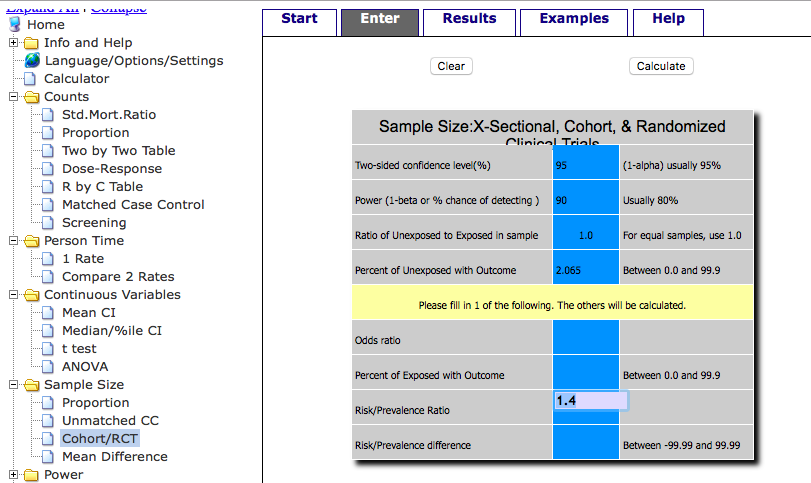
\includegraphics[width=\textwidth]{images/open_epi_example} \end{center}

\end{frame}

\begin{frame}{Software-- Example}

\begin{center}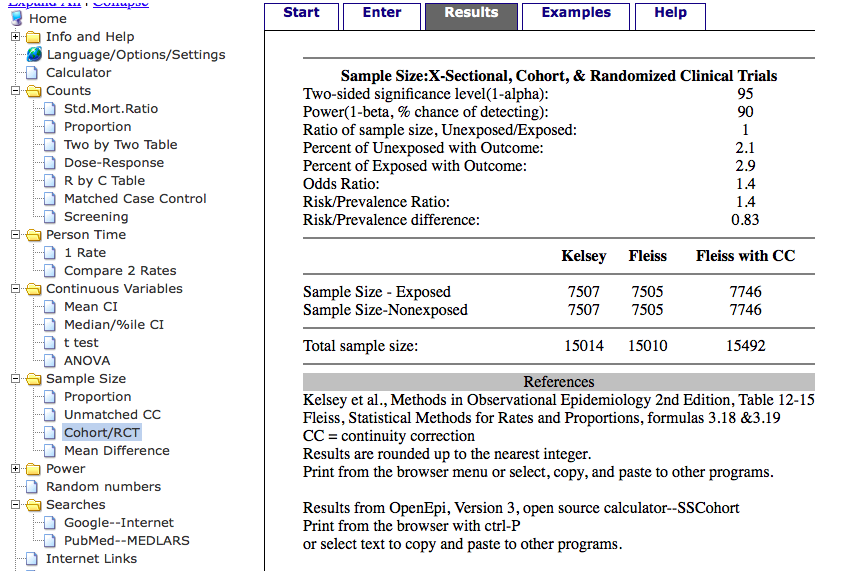
\includegraphics[width=\textwidth]{images/open_epi_results} \end{center}

\end{frame}

\begin{frame}{Required information-- Testing an odds ratio in a
case-control study}

The required inputs for a power calculation or sample size determination
for a hypothesis test testing an odds ratio for an unmatched
case-control study are (you need all but one):

\begin{itemize}
\tightlist
\item
  Number of controls
\item
  Number of cases \emph{or} ratio of controls to cases
\item
  Percent of controls that are exposed
\item
  Percent of cases that are exposed \emph{or} odds ratio
\item
  Desired Type I error rate
\item
  Desired power
\end{itemize}

\end{frame}

\begin{frame}{Required information-- Testing an odds ratio in a
case-control study}

Some software can also calculate power or required sample size for tests
of an odds ratio in a case-control study when the analysis will adjust
for confounders.

However, as the planned analysis gets more complex, the number of inputs
required increases. In this case, the software would also require inputs
of additional assumptions, including the probability of exposure at
different levels of each confounder, the probability of a participant
being in different levels of the confounder, and the odds ratio of
disease and confounder level.

\footnotesize{Edwardes (2001) Sample size requirements for case-control study designs. \textit{BMC Medical Research Methodology} 1:11.}

\end{frame}

\begin{frame}{Getting required information for power calculations}

\begin{itemize}
\tightlist
\item
  Type I error rate (\(\alpha\)) is commonly set to 0.05. Values of 0.01
  or 0.001 are also used sometimes.
\item
  Power is often set to 0.80, 0.90, or 0.95.
\item
  Power and the Type I error rate can be selected based on the risks and
  rewards of the study. For example, a higher rate of Type I error may
  be acceptable, and a lower rate of Type II error desired, in a
  clinical trial if the new treatment being tested has low risks and
  high advantages (e.g., few side effects, low cost, and better efficacy
  than the standard treatment).
\end{itemize}

\end{frame}

\begin{frame}{Getting required information for power calculations}

\begin{itemize}
\tightlist
\item
  For estimates of baseline prevalence, or estimates of variance in
  continuous measurements, you can try to find relevant estimates in the
  literature
\item
  You could also try to estimate these values in a pilot study
\item
  For estimates of the effect size you would like to detect, you should
  consult with subject matter expertise. An important question is what
  result would be medically or clinically significant?
\item
  For all parameters of the power test, it may make sense to test a few
  reasonable values and see how much the calculated power or required
  sample size changes.
\end{itemize}

\end{frame}

\begin{frame}{Getting required information for power calculations}

Schulz and Grimes give an example of the difficulty of collecting
required information:

\begin{quote}
``We needed to estimate an event rate for pelvic inflammatory disease in
users of intrauterine devices in a family planning population in
Nairobi, Kenya. Government officials estimated 40\%; the clinicians at
the medical center thought that estimate was much too high and instead
suggested 12\%. We conservatively planned on 6\%, but the placebo group
in the actual randomised trial yielded 1.9\%. The first estimate was off
by more than 20-fold, which enormously affects sample size
calculations.''
\end{quote}

\footnotesize{Schulz and Grimes. (2005) Sample size calculations in randomised trials: mandatory and mystical. \textit{Lancet} 365:1348--53.}

\end{frame}

\begin{frame}{Rules of thumb and simulations}

With more complex study designs or planned analysis, it may be hard to
find either a formula or software that can be used for an appropriate
power calculation.

\begin{itemize}
\tightlist
\item
  Complex sampling design (stratified sampling, cluster sampling)
\item
  Samples that violate the independence assumption
\item
  Analyses that will adjust for confounding or test interactions
\item
  Analyses that will incorporate many hypothesis tests (e.g., 'omics
  studies)
\end{itemize}

In some cases, statisticians have developed ``rules of thumb'' to
provide guidance in more complex power calculations. In other cases, the
only approach may be a simulation study, and even that might be very
complex to conduct.

\end{frame}

\begin{frame}{Rules of thumb and simulations}

\begin{block}{Cluster sampling}
Section 8.8 of the reading for today gives a rule of thumb for sample size determination when the data was collected using cluster sampling, by calculating and using a design effect (\textit{deff}). The steps are: 
\begin{enumerate}
  \item Determine the sample size required if the data were collected as a simple random sample. 
  \item Calculate the design effect (\textit{deff}) for the sampling. This is a function of the number of individuals per cluster and the intracluster correlation coefficient. 
  \item Increase the estimate of the required sample size by a factor of the value calculated for deff. 
\end{enumerate}
\end{block}

\end{frame}

\begin{frame}{Rules of thumb and simulations}

A few rules of thumb exist for sample size determination when including
confounders in the planned data analysis.

\begin{block}{Rule of 10}
For logistic and Cox regression, include at least 10 \textit{events} (e.g., in a study of risk of mortality, at least 10 deaths) per predictor variable. 
\footnotesize{Vittinghoff and McCulloch. (2007) Relaxing the rule of ten events per variable in logistic and Cox regression. \textit{American Journal of Epidemiology} 165:710--718.}
\end{block}

\begin{block}{From Section 8.9 of reading}
\begin{enumerate}
  \item Determine the sample size if the data analysis were going to be unadjusted
  \item Multiply this estimated sample size by $\frac{1}{1-R^2}$, where $R^2$ is the coefficient of determination from a regression model of the index variable regressed on the confounders. 
\end{enumerate}
\end{block}

\end{frame}

\begin{frame}{Rules of thumb and simulations}

Keep in mind that these rules of thumb are very, very broad guidelines.
They may provide a useful back-of-the-envelope check, but you shouldn't
put heavy weight on them.

In theory, a simulation study could be conducting to determine the power
or calculate the required sample size for almost any study. However, as
the study design and planned analysis increase in complexity, the
simulation would require more and more assumptions and inputs.

\end{frame}

\begin{frame}{Take-home messages}

\begin{center}
\includegraphics[width=0.6\textwidth]{images/type_I_error} \end{center}

\begin{itemize}
  \item Hypothesis tests are not infallible. Type I error rates ($\alpha$) and Type II error rates ($\beta$) give probabilities of how often we expect a hypothesis test to fail in one of the two ways it can fail.
\end{itemize}

\end{frame}

\begin{frame}{Take-home messages}

\begin{itemize}
\tightlist
\item
  Results of power tests and sample size determinations are
  \textbf{ballpark} estimates. They rely on many assumptions that may
  not be appropriate. They are also probabilities, so they give no
  guarantee that a study will result in rejecting the null, even if
  there is a true effect.
\item
  Power tends to increase with increased sample size, increased size in
  the effect to detect, and decreased variance in the observations.
\item
  Different equations and tools should be used for different study
  designs and analysis plans. Many of the available tools are limited to
  fairly simple study designs and analysis plans.
\item
  If you need to do a power calculation for a complex study design or
  analysis plan, review current literature and / or talk to a
  statistician.
\end{itemize}

\end{frame}

\begin{frame}{In-class exercise}

Your research group will be given a pair of dice. You want to test if
they are trick dice (rather than regular dice). If they are trick dice,
you expect to role a 7 50\% of the time (Group 1) or to roll an 11 50\%
of the time (Group 2).

\begin{itemize}
\tightlist
\item
  Decide how you plan to conduct a study. What will you do to collect
  data?
\item
  Decide on the hypothesis test you will conduct. What are your null and
  alternative hypotheses? What is an appropriate test statistic and how
  will you calculate it?
\item
  For a power analysis, what is the effect size you want to be able to
  detect (i.e., what is your value for \(d\))?
\end{itemize}

\end{frame}

\begin{frame}{In-class exercise}

\begin{itemize}
\tightlist
\item
  If you roll the dice 10 times, what is the estimated power of your
  study?
\item
  How many times do you need to roll the dice to conduct a study with
  95\% power?
\item
  For a given number of dice rolls, whose study will have more power,
  your group's or the other group's? Why?
\end{itemize}

\end{frame}

\end{document}
